\chapter{Used Technologies}
\label{chapter:ConfTechnology}
Before the problem can be explained the technologies in question
and the terminology that is used in the rest of this document is in order must first be introduced. This should
only serve as a brief outline since a full explanation goes beyond the scope of this
thesis.

\section{Eclipse}
\label{section:ConfTechEclipse}
\index{Eclipse}
Since the \ac{KIELER} project and thus the Execution Manager is build upon the 
Eclipse framework a short introduction into Eclipse is necessary.

The basic function of Eclipse is as an \ac{IDE} for Java. It provides
a host of facilities that makes it easier for the user to create their own Java applications.
A few examples for these facilities are:
\begin{itemize}
 \item Syntax highlighting to make the source code easier to read.
 \item Automatic completion of partial commands to ensure correctness
and make it easier to write code.
 \item Content assist to create better code and remove errors.
 \item Several wizards for class creation and other tasks.
\end{itemize}

However since Eclipse is an open-source project there are also plug-ins (see Section 
\ref{section:ConfTechPlugins}) for variety of other things. 
For example the language isn't limited to Java. There are also plug-ins
for C++, \LaTeX, Visual Basic and several other programming languages.

Through the use of different modeling framework Eclipse can also be used as an \ac{IDE}
for \ac{IDE}s. That makes Eclipse ``an IDE for anything, and nothing in particular'' \cite{eclipseOverview}.

\begin{figure}
  \centering
  \includegraphics[scale=.25]{EclipseScreen.png}
  \caption[The Eclipse workbench window]%
  {The Eclipse workbench window\protect}
  \label{fig:EclipseScreen}
\end{figure}
The terminology used for the different basic parts of Eclipse can be illustrated based on Figure
\ref{fig:EclipseScreen}:
\begin{itemize}
 \item The main window of Eclipse is called the \textit{workbench}. The workbench consists of the 
different editors and views.
 \item The files that the user operates on are located in the Eclipse \textit{workspace}. 
 \item An \textit{editor} is a component that allows the user to display, enter and modify information.
Editors are used to modify a specific file type. There can usually be multiple instances of the same editor.
An example for an editor would be the Java editor which is used to create and edit Java source files.
 \item An Eclipse \textit{view} is the other component located on the workbench. Views are only used to
display content that was created elsewhere. Unlike editors there is usually only one instance of any view.
One of the views shown in the figure is the class outline view. It shows all methods and attributes of the 
Java class in the currently active editor.
\end{itemize}

For additional information about eclipse see the official Eclipse website\footnote{www.eclipse.org} or literature \cite{eclipsePlugins}.

\subsection{Plug-ins}
\label{section:ConfTechPlugins}
\index{Plug-in}
The building blocks of any Eclipse application are the so called \textit{plug-ins}. They
consist of any number of Java classes and additional meta information. The Java classes
describe the behavior of the plug-in and define its \ac{API}. The meta information is not written
in Java but uses an \ac{XML} notation instead. The meta information contains the following
information:
\begin{itemize}
 \item What other plug-ins does the plug-in depend on? This information is necessary to determine
which other plug-ins have to be loaded or when to refuse loading the plug-in because of missing
dependencies.
 \item What \textit{extension points} does the plug-in offer? These are part of the \ac{API} and
will be described below.
 \item What functionality does it add to the plug-ins which it extends?
\end{itemize}

Plug-ins encapsulate their internal behavior and can be accessed through the \ac{API} and the 
\textit{extension points}. They provide a specific functionality that can be reused as long as
the dependencies are met. As such an Eclipse application consists of a mosaic of different
plug-ins that can be exchanged at will.

Eclipse can not only be used to create plug-ins that can be used in an Eclipse
instance but can also compile a set of plug-ins into a standalone application - the so
called \ac{RCA}. This \ac{RCA} contains a minimal set of plug-ins to provide the Eclipse
look-and-feel and the plug-ins created by the user.

\subsubsection{Extension Point Mechanism}
\label{section:ConfTechExtension}
\index{Extension point}
The extension point mechanism is one of the key features of plug-in development in Eclipse.
It extends the \ac{API} provided by the public methods of the different Java classes inside
the plug-in. An extension point definition consists of a tree of different configuration elements.
Each configuration element has different attributes some of which can be optional while other
are mandatory. These attributes can be anything from a String, a file to a Java class that has
to extend one class and implement a specific interface.

A plug-in that wants to add their functionality to an already existing plug-in
through the use of an extension point has to provide the mandatory attributes defined in the 
specifications.

Eclipse itself already provides many extension points to extend the functionality of the workbench.
For example, if a plug-in wants to add a new editor to the workbench it has to extend the 
\textit{org.eclipse.ui.editors} extension point. It then has to provide an identifier and a name
as well as a class that implements the \textit{org.eclipse.ui.IEditorPart} interface. It can also specify an
icon and a file extension for files which should be opened with the new editor.

When an Eclipse application is started with this plug-in Eclipse will automatically make sure that the new editor
can be used to open the specified file type. The programmer only has to concern himself with the area of the editor
itself without worrying about it being added at all the necessary places inside the Eclipse architecture.

\subsection{Preference Pages}
\label{section:TechPreferencePage}
\index{Preference Page}
A special example of plug-in usage within the Eclipse framework itself is the 

\textit{org.eclipse.ui.preferencePage} plug-in. 
It is used to create new preference pages at a specific location inside the
normal tree of preference pages accessible through Window->Preferences.
The programmer only has to take care of the contents of the actual page and not worry
about additional buttons or integrating it into the PreferenceDialog.

\subsubsection{Preference Store}
\label{section:TechPreferenceStore}
Closely coupled with the preference pages is the Eclipse preference store. It is
basically a text file for each plug-in where the plug-in can deposit simple Strings
under a given key to ensure that information is kept between execution runs.

\section{The KIELER Execution Manager}
\label{section:introKiem}
\index{Execution Manager}
\begin{figure}
  \centering
  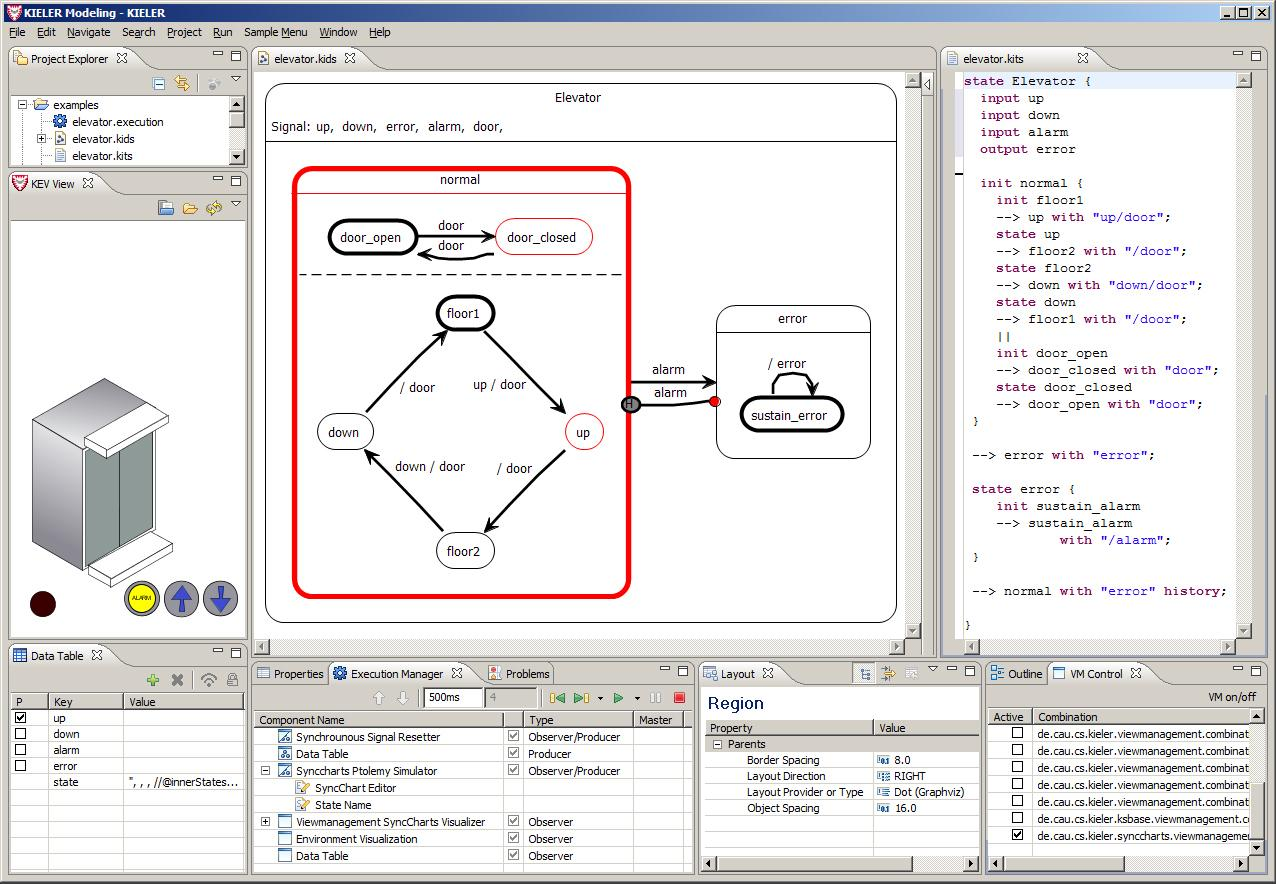
\includegraphics[scale=.3]{KIEMOriginal.jpeg}
  \caption[The Execution Manager during a simulation.]%
  {The Execution Manager during a simulation.\protect}
  \label{fig:KIEMOriginal}
\end{figure}
Execution Manager shown in Figure \ref{fig:KIEMOriginal} is used in \ac{KIELER} as a framework 
to plug-in DataComponents (see Section \ref{section:IntroDataComponent}) for various tasks. Examples are:
\begin{itemize}
 \item Simulation Engines
 \item Model Visualizers
 \item Environment Visualizers
 \item Validators
 \item User Input Facilities
 \item Trace Recording Facilities 
\end{itemize}

These DataComponents can be executed using a graphical user interface (GUI). 
The scheduling order can also be defined by this GUI as well as other settings like a step/tick duration and properties of DataComponents.
For information about \ac{KIEM} see the wiki\footnote{\url{http://rtsys.informatik.uni-kiel.de/trac/kieler/wiki/Projects/KIEM}}.

\subsection{KiemProperty}
\label{section:IntroKiemProperty}
The basic KiemProperty object holds a (key, value) pair of type String. It is used to store information
inside the DataComponents. There are also advanced KiemProperties which can contain other types of values
like integers, booleans or files.

\subsection{DataComponents}
\label{section:IntroDataComponent}
\index{DataComponent}
A DataComponent is an entity that has a specific task during a the course of an execution. The
DataComponents are scheduled in a specific order and can either receive or produce information or both. 
During each step of the execution each DataComponent is asked to perform their computations for the step. Every
DataComponent contains a list of KiemProperties that are used to allow some configuration of the component
after it has been loaded.

\subsubsection{DataComponentWrappers}
\label{section:IntroDataComponentWrapper}
\index{DataComponentWrapper}
A DataComponentWrapper is an object that wrapps around a DataComponent. The wrappers are stored in the schedule
of an execution file.

\subsection{Execution}
\label{section:IntroExecution}
\index{Execution file}
\index{Execution}
\index{Schedule}
The files used by the Execution Manager are called \textit{execution files}. These files contain 
the list of DataComponents with all internal data and the specific order. That list is called a
\textit{schedule}. The schedule can be used to start an \textit{execution} in the Execution Manager.
An execution consists of a initialization, stepping and wrap-up.

\subsection{Model Files}
\label{section:IntroModelFile}
\index{Model file}
\begin{figure}
  \centering
  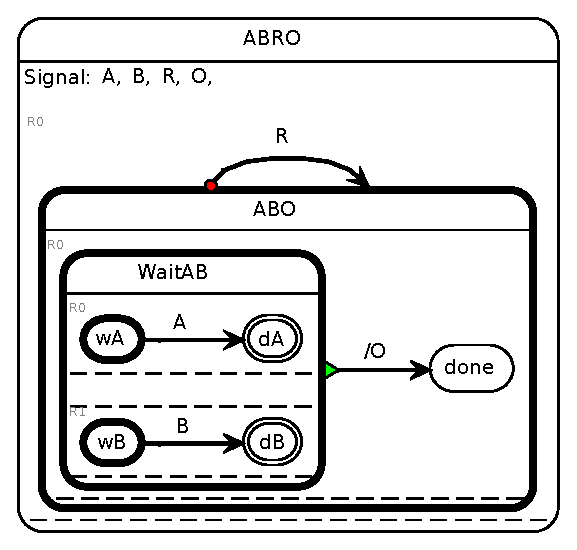
\includegraphics[scale=.8]{abro.pdf}
  \caption[An example for a simple syncchart diagram.]%
  {An example for a simple syncchart diagram.\protect}
  \label{fig:abro}
\end{figure}
A model file is not a concept of the Execution Manager as such but rather a general concept. However
since this thesis only uses model files in the context of the \ac{KIEM} it seems appropriate to explain
them here.

A model file can be any file that contains the structure and behavior of a semantic entity. This can be something as
simple as a text file containing a list of elements in a certain order. Most model files that are used in
the \ac{KIELER} project are diagrams that consist of nodes and links. These \textit{synccharts} are build in
a hierarchical structure and are therefore stored as a tree of different elements. For an example of a simple
syncchart see Figure \ref{fig:abro}.

\section{Related Work}
\label{section:RelatedWork}
There are of course a huge amount of other applications and projects that deal
with configuration management. In order to get some idea of similar projects
a few examples from Eclipse itself and the \ac{KIELER} project will be used.

\subsection{Configurations}
\label{section:RelatedConf}
\index{Configuration}
One of the tasks that will be explained in Section \ref{section:ConfTaskConfig} is to add new
configuration information to existing execution files. This task can be compared to
the \ac{KIML} project. 

\ac{KIML} is used to automatically layout existing diagrams. Since diagrams basicly consist of nodes and
connections generic algorithms can be used to layout almost any type of diagram. However the user still
has some control over the details of the automatic layout process. The user can configure details like
the distance between different elements, the direction of the layout or the layouter that should be used.

This meta-information has to be stored somewhere. The approach used in \ac{KIML} was to create a separate
file. The file has the same name as the diagram file and contains all the layout information needed for it.
The information can be easily reset by deleting the separate file. 
